\documentclass[11pt, letterpaper]{article}

% --- PREÁMBULO ---
\usepackage[utf8]{inputenc}
\usepackage[T1]{fontenc}
\usepackage[letterpaper, top=2.2cm, bottom=2.2cm, left=2.2cm, right=2.2cm]{geometry}
\usepackage{xcolor}
\usepackage{graphicx}
\usepackage[most]{tcolorbox}
\usepackage{enumitem}
\usepackage{tikz}
\usepackage{booktabs}
\usepackage{fancyhdr}
\usepackage{eso-pic} % AÑADIDO: Necesario para \AddToShipoutPictureBG*

% --- COLORES INSTITUCIONALES ---
\definecolor{valblue}{RGB}{0,112,192}
\definecolor{valdark}{RGB}{30,30,30}
\definecolor{valgray}{RGB}{240,240,240}

% --- FUENTE ---
\usepackage{helvet}
\renewcommand{\familydefault}{\sfdefault}

% --- CONFIGURACIÓN DE PÁGINA ---
\pagestyle{fancy}
\fancyhf{}
\fancyhead[L]{\footnotesize \color{gray} LICEO V.A.L. -- MATEMÁTICAS 6º}
\fancyhead[R]{\footnotesize \color{gray} CÓDIGO: 06M-17}
\fancyfoot[C]{\footnotesize \color{gray} Página \thepage}
\renewcommand{\headrulewidth}{0.4pt}
\renewcommand{\footrulewidth}{0pt}

% --- CONFIGURACIÓN DE RESPUESTAS ---
\newif\ifshowanswers
\showanswerstrue % Cambiar a \showanswersfalse para la versión del estudiante

\newcommand{\cono}{\tikz[scale=0.15]{
		\draw[fill=orange!30, draw=orange!60!black, line width=0.1pt] (0,0) -- (1,0) -- (0.5,-1.5) -- cycle; 
		\draw[fill=red!50, draw=red!70!black, line width=0.1pt] (0.5,0.25) circle (0.45);
}}

\newcommand{\answer}[1]{
	\ifshowanswers
	\par\vspace{0.2cm}
	\begin{tcolorbox}[colback=blue!5!white, colframe=blue!60!white, arc=1mm, boxrule=0.5pt, title=\textbf{\footnotesize SOLUCIÓN (DOCENTE)}]
		\color{blue!80!black}\footnotesize #1
	\end{tcolorbox}
	\par\vspace{0.2cm}
	\else
	\par\vspace{0.3cm}
	\fi
}

\begin{document}
	
	% --- CAPA DE AGUA DE FONDO (Si existe el archivo) ---
	\IfFileExists{../../FondoVAL.pdf}{
		\AddToShipoutPictureBG*{
			
\includegraphics[width=\paperwidth,height=\paperheight,keepaspectratio=false]{../../FondoVAL.pdf}
		}
	}{}
	
	% --- ENCABEZADO ---
	\begin{center}
		{\Large \textbf{\color{valblue} LICEO V.A.L.}}\\[0.1cm]
		{\large \textbf{Taller de Repaso -- Trabajo en Cuaderno}}\\[0.1cm]
		{\small \textbf{Materia: Matemáticas 6º} \quad | \quad \textbf{Unidad: Lectura de Gráficas y Tablas} \quad | \quad \textbf{Código: 06M-17}}
	\end{center}
	
	\vspace{0.2cm}
	\noindent \textbf{Nombre del Estudiante:} \underline{\hspace{8cm}} \hfill \textbf{Fecha:} \underline{\hspace{3cm}}
	
	\vspace{0.4cm}
	\begin{tcolorbox}[colback=valgray, colframe=valdark, arc=1mm, boxrule=0.8pt]
		\textit{Instrucciones: Transcribe y resuelve cada uno de los siguientes 5 puntos en tu cuaderno de matemáticas de forma ordenada. No es necesario calcar todas las gráficas, pero sí debes escribir los procedimientos y justificaciones correspondientes.}
	\end{tcolorbox}
	
	\vspace{0.4cm}
	
	% --- PREGUNTAS ---
	
	\noindent \textbf{1. (20\%)} Una persona desea enviar un paquete de 3 lb a la Zona 4 de correo prioritario, y otro paquete de 1 lb a la Zona 3. Utilizando la siguiente tabla de tarifas postales de 2017 de tu libro de texto, calcula el costo total del envío de ambos paquetes:
	
	\begin{center}
		\begin{tabular}{ccccc}
			\toprule
			\textbf{Peso} & \textbf{Zonas 1 y 2} & \textbf{Zona 3} & \textbf{Zona 4} & \textbf{Zona 5} \\
			\midrule
			1 lb & \$5,75 & \$6,26 & \$6,37 & \$6,53 \\
			2 lb & \$6,33 & \$6,40 & \$6,63 & \$7,91 \\
			3 lb & \$6,41 & \$7,16 & \$7,62 & \$9,22 \\
			4 lb & \$6,62 & \$7,39 & \$8,46 & \$10,19 \\
			\bottomrule
		\end{tabular}
	\end{center}
	
	\answer{
		Buscamos los valores en la tabla por intersección de fila (peso) y columna (zona):\\
		- Paquete de 3 lb enviado a la Zona 4: \textbf{\$7,62}\\
		- Paquete de 1 lb enviado a la Zona 3: \textbf{\$6,26}\\
		Costo total = \$7,62 + \$6,26 = \textbf{\$13,88}
	}
	
	\vspace{0.5cm}
	
	\noindent \textbf{2. (20\%)} Observa la siguiente gráfica de barras que muestra la velocidad máxima estimada para algunos animales según tu libro de Cengage. ¿Cuál es la diferencia de velocidad, en millas por hora (mph), entre el animal más rápido de la gráfica y el coyote?
	
	\begin{center}
		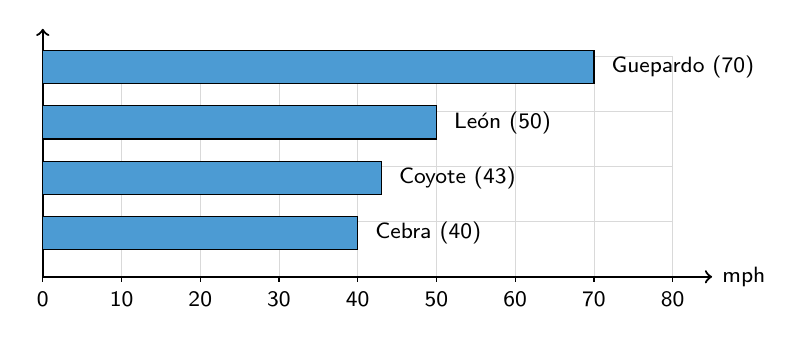
\begin{tikzpicture}[yscale=0.7]
			\draw[very thin, gray!30] (0,0) grid (8,4);
			\draw[thick, ->] (0,0) -- (8.5,0) node[right] {\footnotesize mph};
			\draw[thick, ->] (0,0) -- (0,4.5);
			\foreach \x in {0,10,20,30,40,50,60,70,80} {
				\draw (\x/10, 0) -- (\x/10, -0.1) node[below] {\footnotesize \x};
			}
			\draw[fill=valblue!70, draw=black] (0,3.5) rectangle (7.0, 4.1);
			\node[right] at (7.1, 3.8) {\footnotesize Guepardo (70)};
			\draw[fill=valblue!70, draw=black] (0,2.5) rectangle (5.0, 3.1);
			\node[right] at (5.1, 2.8) {\footnotesize León (50)};
			\draw[fill=valblue!70, draw=black] (0,1.5) rectangle (4.3, 2.1);
			\node[right] at (4.4, 1.8) {\footnotesize Coyote (43)};
			\draw[fill=valblue!70, draw=black] (0,0.5) rectangle (4.0, 1.1);
			\node[right] at (4.1, 0.8) {\footnotesize Cebra (40)};
		\end{tikzpicture}
	\end{center}
	
	\answer{
		- Identificamos la velocidad del animal más rápido (el de la barra más larga): \textbf{Guepardo = 70 mph}.\\
		- Identificamos la velocidad de la barra del coyote: \textbf{Coyote = 43 mph}.\\
		- Calculamos la diferencia realizando una resta simple: 70 - 43 = \textbf{27 mph}.
	}
	
	\newpage
	
	\noindent \textbf{3. (20\%)} En la heladería \textit{Barney's Café}, se registró la venta diaria de helados de diferentes poblaciones a través de un pictograma. Si cada símbolo \cono\ equivale a \textbf{\$100}, ¿cuánto dinero en total gastaron los niños y los ancianos juntos en helados?
	
	\begin{center}
		\begin{tabular}{rl}
			\toprule
			\textbf{Grupo de Clientes} & \textbf{Ventas de Helados (Cada \cono\ = \$100)} \\
			\midrule
			Niños: & \cono\ \cono\ \cono\ \cono\ \cono \\
			Padres: & \cono\ \cono\ \cono\ \cono \\
			Ancianos: & \cono\ \cono \\
			\bottomrule
		\end{tabular}
	\end{center}
	
	\answer{
		- Contamos los símbolos para cada uno de los grupos indicados:\\
		* Niños: 5 símbolos $\rightarrow$ 5 $\times$ \$100 = \$500.\\
		* Ancianos: 2 símbolos $\rightarrow$ 2 $\times$ \$100 = \$200.\\
		- Sumamos el total de dinero gastado por ambos grupos: \$500 + \$200 = \textbf{\$700}.\\
		*(O de forma equivalente: 5 + 2 = 7 símbolos en total; 7 $\times$ \$100 = \textbf{\$700}).
	}
	
	\vspace{0.5cm}
	
	\noindent \textbf{4. (20\%)} Observa la gráfica de líneas que muestra el número de estaciones de esquí en operación en Estados Unidos a lo largo del tiempo. ¿Entre qué dos años consecutivos se registró la mayor disminución en el número de estaciones y de cuánto fue esa disminución?
	
	\begin{center}
		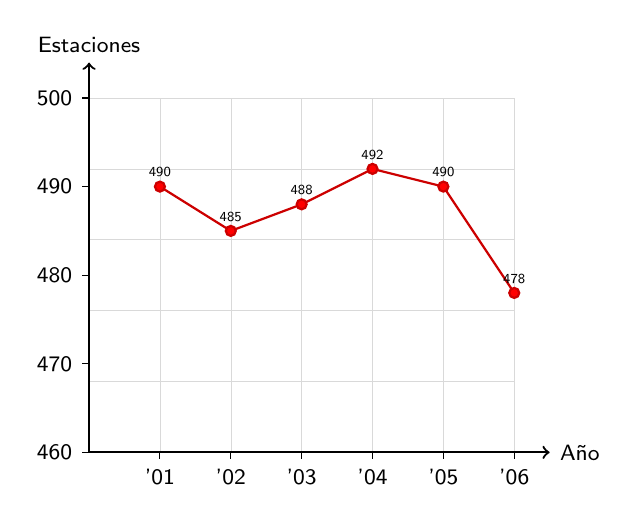
\begin{tikzpicture}[scale=0.9]
			\draw[very thin, gray!30] (0,0) grid (6,5);
			\draw[thick, ->] (0,0) -- (6.5,0) node[right] {\footnotesize Año};
			\draw[thick, ->] (0,0) -- (0,5.5) node[above] {\footnotesize Estaciones};
			\foreach \x/\label in {1/'01, 2/'02, 3/'03, 4/'04, 5/'05, 6/'06} {
				\draw (\x, 0) -- (\x, -0.1) node[below] {\footnotesize \label};
			}
			\foreach \y/\val in {0/460, 1.25/470, 2.5/480, 3.75/490, 5/500} {
				\draw (0, \y) -- (-0.1, \y) node[left] {\footnotesize \val};
			}
			\draw[thick, red!80!black, mark=*, mark options={fill=red}] plot coordinates {
				(1, 3.75) (2, 3.125) (3, 3.5) (4, 4.0) (5, 3.75) (6, 2.25)
			};
			\node[above] at (1, 3.75) {\tiny 490};
			\node[above] at (2, 3.125) {\tiny 485};
			\node[above] at (3, 3.5) {\tiny 488};
			\node[above] at (4, 4.0) {\tiny 492};
			\node[above] at (5, 3.75) {\tiny 490};
			\node[above] at (6, 2.25) {\tiny 478};
		\end{tikzpicture}
	\end{center}
	
	% AÑADIDO: Bloque de respuesta faltante
	\answer{
		- Primero, observamos en la gráfica los años donde el número de estaciones disminuyó y calculamos la diferencia:\\
		* De '01 a '02: $490 - 485 = 5$ estaciones.\\
		* De '04 a '05: $492 - 490 = 2$ estaciones.\\
		* De '05 a '06: $490 - 478 = 12$ estaciones.\\
		- Concluimos que la mayor disminución se registró entre los años \textbf{'05 y '06}, con una caída de \textbf{12 estaciones}.
	}
	
	\vspace{0.5cm}
	
	\noindent \textbf{5. (20\%)} El siguiente histograma muestra la cantidad de millas de trayecto por semana recorridas por los empleados de una compañía de seguros. ¿Cuántos empleados recorren un trayecto semanal que está comprendido en los intervalos de \textbf{4,5 a 14,5 millas}?
	
	\begin{center}
		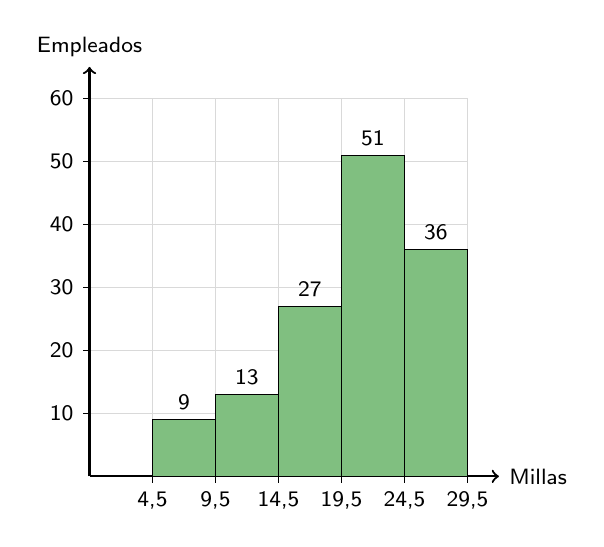
\begin{tikzpicture}[scale=0.8]
			\draw[very thin, gray!30] (0,0) grid (6,6);
			\draw[thick, ->] (0,0) -- (6.5,0) node[right] {\footnotesize Millas};
			\draw[thick, ->] (0,0) -- (0,6.5) node[above] {\footnotesize Empleados};
			
			% CORREGIDO: Las variables numéricas con comas deben estar entre llaves { }
			\foreach \x/\label in {1/{4,5}, 2/{9,5}, 3/{14,5}, 4/{19,5}, 5/{24,5}, 6/{29,5}} {
				\draw (\x, 0) -- (\x, -0.1) node[below] {\footnotesize \label};
			}
			\foreach \y/\val in {1/10, 2/20, 3/30, 4/40, 5/50, 6/60} {
				\draw (0, \y) -- (-0.1, \y) node[left] {\footnotesize \val};
			}
			\draw[fill=green!50!black!50, draw=black] (1,0) rectangle (2, 0.9);
			\draw[fill=green!50!black!50, draw=black] (2,0) rectangle (3, 1.3);
			\draw[fill=green!50!black!50, draw=black] (3,0) rectangle (4, 2.7);
			\draw[fill=green!50!black!50, draw=black] (4,0) rectangle (5, 5.1);
			\draw[fill=green!50!black!50, draw=black] (5,0) rectangle (6, 3.6);
			
			\node[above] at (1.5, 0.9) {\footnotesize 9};
			\node[above] at (2.5, 1.3) {\footnotesize 13};
			\node[above] at (3.5, 2.7) {\footnotesize 27};
			\node[above] at (4.5, 5.1) {\footnotesize 51};
			\node[above] at (5.5, 3.6) {\footnotesize 36};
		\end{tikzpicture}
	\end{center}
	
	\answer{
		El trayecto total de 4,5 a 14,5 millas comprende los primeros dos intervalos del histograma:\\
		- Intervalo 4,5 - 9,5: \textbf{9 empleados}\\
		- Intervalo 9,5 - 14,5: \textbf{13 empleados}\\
		Sumamos ambos valores para hallar el total: 9 + 13 = \textbf{22 empleados}.
	}
	
	\vfill
	\begin{center}
		\textit{\color{valdark!70} ``El éxito es la suma de pequeños esfuerzos repetidos día tras día.''}
	\end{center}
	
\end{document}